\documentclass[final,5p,times,twocolumn]{elsarticle}

% Edited sections are local; figures, tables and appendices are shared.
\graphicspath{{./}}

\usepackage[T1]{fontenc}
\usepackage[utf8]{inputenc}
\usepackage{lmodern}
\usepackage{amsmath,amssymb,booktabs,graphicx,tabularx}
\usepackage{array}
\usepackage{xcolor,tikz,pgfplots}
\usetikzlibrary{arrows.meta,positioning,fit,shapes.geometric,calc}
\pgfplotsset{compat=1.18}
\usepackage{etoolbox}
% Compact table typography for the narrow two-column measure.
\AtBeginEnvironment{tabular}{\scriptsize\setlength{\tabcolsep}{2pt}}
\AtBeginEnvironment{tabularx}{\footnotesize\setlength{\tabcolsep}{3pt}}
\usepackage[hidelinks]{hyperref}
\usepackage{xurl}
\usepackage{microtype}
\usepackage{flushend}
\setlength{\emergencystretch}{1.5em}
% Let full-width floats move to a suitable page top.  Cross-references keep the
% discussion unambiguous without forcing each figure into its source section.
\usepackage{placeins}
\setlength{\belowcaptionskip}{6pt}
\newcommand{\authorquery}[1]{\par\smallskip\noindent\textcolor{red!65!black}{\textbf{Author query:} #1}\par\smallskip}

\journal{Chinese Journal of Aeronautics}

\begin{document}
\begin{frontmatter}
\title{DisasterClaw: A task-centric benchmark for active observation in embodied UAV inspection}
\author{Anonymous authors}
\affiliation{organization={Anonymous submission}}
\begin{abstract}
Aerial agents can actively acquire new observations to resolve uncertainty, but doing so incurs sensing and maneuvering costs. Existing evaluations often assess navigation or perception without isolating whether a new observation improves the final answer. To address this gap, we introduce DisasterClaw, a georeferenced benchmark and replay platform for evaluating task-conditioned observation decisions in disaster assessment. DisasterClaw keeps the question, geographic region, and reference answer fixed while allowing vehicle actions to change the observed image footprint. Its traceable evaluation protocol connects observations, predicted evidence, actions, and answers, and uses matched fixed-view controls to distinguish the value of new visual evidence from additional answer calls. The benchmark comprises 160 human-reviewed questions across 44 regions and three disaster events. Text-only and permitted-metadata controls achieve accuracies of 28.75\% and 36.25\%, respectively, compared with 72.29\% and 75.00\% for image-aware policies. Across 161 recheck transitions, changed-view accuracy reaches 59.63\%, versus 50.31\% for matched fixed-view calls, yielding a gain of 9.32 percentage points with a 95\% region-clustered interval of [-2.00, 21.74]. These transitions produce 36 corrections and 21 harms, highlighting both the potential benefits and risks of re-observation. An additional offline case study applies a single-temporal adaptation of the controller to 409 eligible image pairs from MESSI, using existing YOLO and SegFormer models. The controller requests 20 lower-altitude observations, increasing the number of correct answers from 369 to 372; on these triggered cases, lower-altitude observations yield 15 correct answers, compared with 12 under an equal-budget repeat-high control. Together, these experiments provide a reproducible basis for studying when additional observations help aerial agents, while leaving consistent cross-scene gains and physical flight effectiveness unestablished. Project resources will be available at https://github.com/emmmmmmnbbb/DisasterClaw.
\end{abstract}
\begin{keyword}
Embodied aerial agents \sep Active perception \sep Disaster assessment \sep Observation value \sep Benchmarking
\end{keyword}
\end{frontmatter}

\section{Introduction}
Embodied AI for aerospace vehicles links onboard sensing, task reasoning, and executable actions under vehicle and mission constraints. In aerial disaster inspection, an agent may be asked whether a building is damaged, how many damaged buildings lie within a region, or where the nearest damaged building is located. Descending toward a building may improve local detail while narrowing the visible footprint and excluding evidence needed for a regional assessment. The value of an additional observation therefore depends on the question being answered and the maneuver it requires.

Embodied multimodal models connect visual and state observations to task reasoning, while language-guided navigation and vision-language-action systems ground plans in executable skills and actions~\cite{driess2023palme,shah2023lmnav,ichter2023saycan,zitkovich2023rt2}. Aerial navigation and embodied benchmarks evaluate action-conditioned observations and mission behavior; remote-sensing agents support disaster interpretation and structured tool use~\cite{liu2023aerialvln,lee2025citynav,gao2026openfly,yao2024aeroverse,guo2026bedi,zhao2025cityeqa,liu2024rescueadi,thinkgeo2025}. These capabilities motivate an evaluation question that is narrower but consequential: how does a vehicle's decision to acquire a new view affect the answer to a task whose geographic scope and reference remain fixed? Answering it requires a controlled observation change and a trace linking the action to geographic evidence and the answer call. A standardized episode interface can make this comparison repeatable by distinguishing a requested action from an executed movement and separating changed-view effects from another answer opportunity.

We present DisasterClaw, an imagery-based platform and task benchmark for this evaluation problem. Paired xBD tiles, building annotations, task regions, and simulated vehicle states share a common geographic reference. Annotation-derived answers remain fixed as the agent searches or changes its observation footprint. Four task families impose different requirements for local detail, regional coverage, and geographic reference. An operator console supports scene inspection, and a headless runner executes the quantitative evaluation.

The evaluation connects observation changes to building predictions and task answers. A camera-ladder diagnostic on the development set measures how a narrower footprint affects building localization and damage classification, including corrections and harms. On the frozen final set of 160 human-reviewed questions from 44 regions in three events, shortcut controls assess performance using only question text or permitted runtime metadata. A fixed-view matched-call diagnostic then branches at every executed T1 recheck: one branch reruns perception and answering on the previous image, and the other executes the logged recheck. Matching the answer opportunity helps distinguish the effect of changed observations at individual transitions. A separate MESSI case compares real UAV images acquired at two heights with repeat-view and digital-crop controls. We then inventory the full 2,525-image release and select 409 eligible two-height vegetation regions under the fixed protocol. On these pairs, we run a single-temporal adaptation of DisasterClaw with its existing YOLO and SegFormer models; the controller sees only the high view until its recheck gate authorizes the registered lower view. This measures adapted offline re-observation on real UAV imagery, alongside the platform's primary xBD evaluation.

The contributions are:
\begin{enumerate}
\item a georeferenced, ROI-scoped task benchmark in which the reference answer stays fixed as the observation changes, with an explicit boundary between runtime task cues and scoring labels;
\item an inspection interface that records requested and executed actions, rendered views, predicted evidence, answer calls, and terminal outcomes within the same episode; and
\item an empirical characterization of observation value through shortcut controls, fixed-view matched calls, and corrections and harms by task, using a fixed task-conditioned policy as a reference implementation.
\end{enumerate}

The platform renders existing orthographic imagery under simplified motion. We position it as an evaluation component for embodied aerial agents: it measures task-conditioned sensing decisions and answer consequences, while leaving vehicle dynamics, onboard sensing, and physical flight to future evaluation. The findings apply to this controlled observation setting; they do not establish flight effectiveness.

\section{Related work}
\subsection{Aerial interaction and embodied evaluation}
AerialVLN, CityNav, and OpenFly emphasize language-conditioned aerial navigation, while AeroVerse and BEDI broaden evaluation toward perception, spatial reasoning, planning, motion, and perception--decision--action loops~\cite{liu2023aerialvln,lee2025citynav,gao2026openfly,yao2024aeroverse,guo2026bedi}. CityEQA evaluates question answering after active exploration in a realistic urban simulator~\cite{zhao2025cityeqa}. These systems support action-dependent observations and large-scale evaluation of aerial embodied behavior. Several also provide substantially richer 3D simulation, real-world data, or broader embodied tasks than the controlled orthographic setting used here.

\subsection{Disaster and remote-sensing agents}
xBD supplies paired disaster imagery and building-damage annotations~\cite{gupta2019xbd}. RescueADI, ThinkGeo, and DisasterM3 study tool use or multimodal disaster interpretation from remote-sensing records~\cite{liu2024rescueadi,thinkgeo2025,wang2025disasterm3}. These resources motivate disaster-specific questions. Evaluating an answer from a static image, however, does not measure the value of an agent's decision to observe again. DisasterClaw binds question scope, vehicle state, rendered observation, and terminal answer in one record. This binding also exposes a failure mode: a view that improves one building prediction can remove evidence required by a count or spatial question.

Table~\ref{tab:capability-comparison} summarizes the evaluation capabilities most relevant to this distinction. The comparison focuses on evaluation capabilities; it does not rank the overall scope of the benchmarks. Among the compared benchmarks, DisasterClaw explicitly standardizes a fixed annotation-derived geographic task and answer under view change, geographic evidence traces across observations, and a matched fixed-view answer call. These features define its contribution within a controlled observation setting.

\begin{table*}[!t]
\centering
\scriptsize
\caption{Capability-oriented comparison of benchmarks most relevant to task-dependent observation value.}
\label{tab:capability-comparison}
\resizebox{\textwidth}{!}{%
\begin{tabular}{@{}llccccc@{}}
\toprule
Benchmark & Primary task & \shortstack{Active\\view change} & \shortstack{Disaster-\\specific} & \shortstack{Fixed geographic\\task/answer\\under view change} & \shortstack{Answer after\\active sensing} & \shortstack{Explicit observation-\\value isolation}\\
\midrule
AerialVLN & Aerial vision--language navigation & $\checkmark$ & --- & --- & --- & ---\\
OpenFly & Large-scale aerial vision--language navigation & $\checkmark$ & --- & --- & --- & ---\\
BEDI & UAV embodied-agent evaluation & $\checkmark$ & $\triangle$ & --- & $\triangle$ & ---\\
CityEQA & Embodied question answering & $\checkmark$ & --- & $\triangle$ & $\checkmark$ & ---\\
RescueADI & Disaster remote-sensing agent & --- & $\checkmark$ & --- & $\triangle$ & ---\\
ThinkGeo & Tool-augmented remote-sensing agent & $\triangle$ & $\triangle$ & --- & $\triangle$ & ---\\
DisasterM3 & Disaster vision--language benchmark & --- & $\checkmark$ & --- & --- & ---\\
\textbf{DisasterClaw} & Disaster inspection and observation-value measurement & $\checkmark$ & $\checkmark$ & $\checkmark$ & $\checkmark$ & $\checkmark$\\
\bottomrule
\end{tabular}}
\vspace{2pt}
\parbox{\textwidth}{\footnotesize ``---'' means that the capability is not the primary evaluation contract reported by the work, rather than that it is technically impossible. $\triangle$ denotes a related but non-equivalent capability. DisasterClaw changes controlled orthographic image footprints rather than physical 3D viewpoints.}
\end{table*}


\subsection{Task value of an observation}
Active perception treats sensing as a task-directed action~\cite{bajcsy1988active}. Entropy and calibrated probabilities can guide such actions, but neither directly measures the correctness of a later task answer~\cite{guo2017calibration,ovadia2019can}. We therefore report localization, answer corrections and harms, executed rechecks, and terminal accuracy separately. The task-conditioned rule in this paper is a fixed heuristic for descending subject to predicted ROI coverage and motion cost. Complete-policy comparisons measure outcomes at the realized operating points. We additionally use fixed-view matched calls at executed recheck transitions to control for the extra answer opportunity and examine the contribution of changed observations and evidence within this diagnostic design.

\section{The DisasterClaw platform}
\label{sec:platform}
\subsection{From geographic records to inspection episodes}
DisasterClaw links each task, observation, and answer to a common geographic scene (Fig.~\ref{fig:overview}). Paired xBD images are positioned with pixel-to-geographic affine transforms. Building polygons and damage labels define the reference task; a vehicle state and observation window determine what the agent can see. The operator console and headless runner share the same scene and controller modules. All reported quantitative results are produced by the headless runner.

\begin{figure*}[!t]
\centering
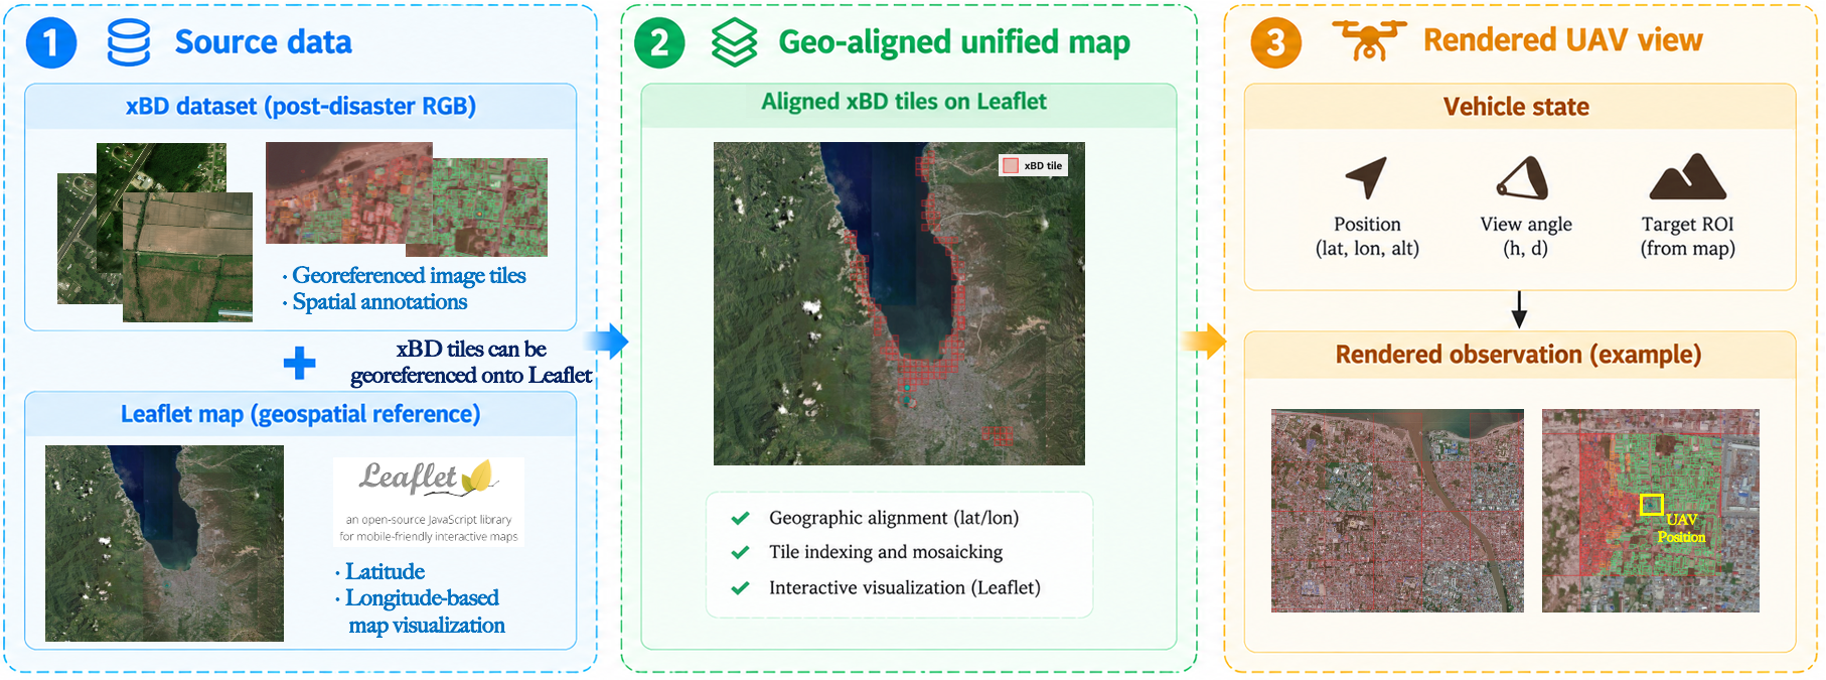
\includegraphics[width=\textwidth]{figure-paper/数据集搭建.png}
\caption{Dataset and scene construction. Georeferenced xBD imagery and spatial annotations are aligned with a Leaflet map, indexed into a unified geographic scene, and rendered according to vehicle state and the target ROI. The basemap supplies geographic context but no damage ground truth.}
\label{fig:overview}
\end{figure*}

The active disaster tile is embedded at its recorded map footprint. Geographic coordinates locate the task ROI, marked building when applicable, vehicle, and rendered window. Disaster imagery supplies the annotated task evidence; a basemap can supply context outside available tiles but contributes no damage ground truth. The task answer remains defined on the ROI when search or recheck changes the observation window. The experiments use this fixed-answer, variable-view design to evaluate observation value.

\subsection{Controlled observation and action}
The nadir renderer uses a $60^\circ$ horizontal field of view and a $1024$-pixel output width. At height $h$, the ground-footprint width $L$ and nominal ground sampling distance $g$ are
\begin{equation}
 L(h)=2h\tan(\theta/2),\qquad g(h)=\frac{L(h)}{W}.
 \label{eq:geometry}
\end{equation}
The assumed source scale is $0.5$ m/pixel, so a $1024$-pixel tile defines a nominal 512 m width. Footprints of three, two, and one tile widths give cruise, intermediate, and floor states at approximately 1330.2, 886.8, and 443.4 m, with nominal GSDs of 1.5, 1.0, and 0.5 m/pixel (Fig.~\ref{fig:ladder}). Geographic placement comes from the recorded affine transforms; the $0.5$ m/pixel value defines the camera ladder without assuming an independently verified physical scale for every source tile.

\begin{figure}[htbp]
\centering
\resizebox{\linewidth}{!}{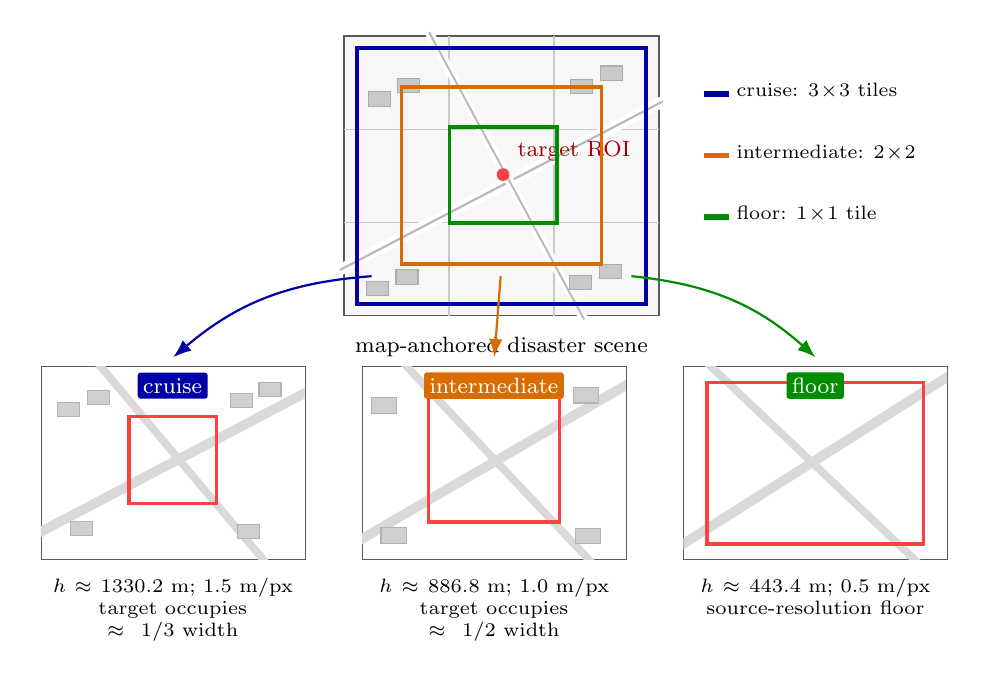
\begin{tikzpicture}[
  font=\footnotesize,
  >=Latex,
  view/.style={draw=black!65,minimum width=3.35cm,minimum height=2.45cm,inner sep=0pt},
  note/.style={align=center,text width=3.45cm,font=\scriptsize}
]
% Source mosaic and nested ground footprints.
\begin{scope}[shift={(3.85,3.55)}]
  \draw[fill=gray!6,draw=black!65] (0,0) rectangle (4.0,3.55);
  \foreach \x in {1.333,2.667}{\draw[gray!42] (\x,0)--(\x,3.55);}
  \foreach \y in {1.183,2.367}{\draw[gray!42] (0,\y)--(4,\y);}
  \draw[line width=4pt,white] (-.05,.58)--(4.05,2.72);
  \draw[line width=.8pt,gray!55] (-.05,.58)--(4.05,2.72);
  \draw[line width=3.2pt,white] (3.05,-.05)--(1.08,3.60);
  \draw[line width=.7pt,gray!55] (3.05,-.05)--(1.08,3.60);
  \foreach \p in {(.45,2.75),(.82,2.92),(3.02,2.91),(3.40,3.08),(3.00,.42),(3.38,.56),(.43,.34),(.80,.49)}{
    \draw[fill=gray!42,draw=gray!65] \p ++(-.14,-.09) rectangle ++(.28,.18);
  }
  \fill[red!75] (2.02,1.79) circle (2.3pt);
  \node[red!65!black,anchor=south west] at (2.08,1.84) {target ROI};
  \draw[line width=1.4pt,blue!65!black] (.17,.15) rectangle (3.83,3.40);
  \draw[line width=1.4pt,orange!85!black] (.73,.65) rectangle (3.27,2.90);
  \draw[line width=1.4pt,green!55!black] (1.34,1.18) rectangle (2.70,2.39);
  \node[anchor=north] at (2,-.15) {map-anchored disaster scene};
\end{scope}

\node[anchor=west,align=left,font=\scriptsize] at (8.30,6.40) {\textcolor{blue!65!black}{\rule{9pt}{2pt}} cruise: $3\!\times\!3$ tiles};
\node[anchor=west,align=left,font=\scriptsize] at (8.30,5.62) {\textcolor{orange!85!black}{\rule{9pt}{2pt}} intermediate: $2\!\times\!2$};
\node[anchor=west,align=left,font=\scriptsize] at (8.30,4.84) {\textcolor{green!55!black}{\rule{9pt}{2pt}} floor: $1\!\times\!1$ tile};

% Three observations have the same output size.
\begin{scope}[shift={(0,0.45)}]
  \node[view,anchor=south west] at (0,0) {};
  \clip (0,0) rectangle (3.35,2.45);
  \draw[line width=3.5pt,gray!30] (-.2,.25)--(3.55,2.22);
  \draw[line width=2.8pt,gray!30] (2.95,-.15)--(.62,2.62);
  \foreach \p in {(.35,1.91),(.73,2.06),(2.55,2.02),(2.91,2.16),(2.64,.36),(.52,.40)}{
    \draw[fill=gray!38,draw=gray!60] \p ++(-.14,-.09) rectangle ++(.28,.18);
  }
  \draw[very thick,red!75] (1.12,.71) rectangle (2.23,1.82);
  \node[fill=blue!65!black,text=white,rounded corners=1pt,inner sep=2pt] at (1.675,2.21) {cruise};
\end{scope}
\node[note,anchor=north] at (1.675,.34) {$h\approx1330.2$ m; 1.5 m/px\\target occupies $\approx1/3$ width};

\begin{scope}[shift={(4.08,0.45)}]
  \node[view,anchor=south west] at (0,0) {};
  \clip (0,0) rectangle (3.35,2.45);
  \draw[line width=3.5pt,gray!30] (-.25,.12)--(3.6,2.36);
  \draw[line width=2.8pt,gray!30] (3.05,-.18)--(.40,2.63);
  \foreach \p in {(.28,1.96),(2.84,2.09),(2.87,.30),(.40,.31)}{
    \draw[fill=gray!38,draw=gray!60] \p ++(-.16,-.10) rectangle ++(.32,.20);
  }
  \draw[very thick,red!75] (.84,.48) rectangle (2.51,2.15);
  \node[fill=orange!85!black,text=white,rounded corners=1pt,inner sep=2pt] at (1.675,2.21) {intermediate};
\end{scope}
\node[note,anchor=north] at (5.755,.34) {$h\approx886.8$ m; 1.0 m/px\\target occupies $\approx1/2$ width};

\begin{scope}[shift={(8.16,0.45)}]
  \node[view,anchor=south west] at (0,0) {};
  \clip (0,0) rectangle (3.35,2.45);
  \draw[line width=3.5pt,gray!30] (-.35,-.02)--(3.7,2.54);
  \draw[line width=2.8pt,gray!30] (3.18,-.23)--(.12,2.67);
  \draw[very thick,red!75] (.30,.20) rectangle (3.05,2.25);
  \node[fill=green!55!black,text=white,rounded corners=1pt,inner sep=2pt] at (1.675,2.21) {floor};
\end{scope}
\node[note,anchor=north] at (9.835,.34) {$h\approx443.4$ m; 0.5 m/px\\source-resolution floor};

\draw[->,thick,blue!65!black] (4.20,4.05) to[bend right=18] (1.68,3.02);
\draw[->,thick,orange!85!black] (5.84,4.05) -- (5.76,3.02);
\draw[->,thick,green!55!black] (7.50,4.05) to[bend left=18] (9.84,3.02);
\end{tikzpicture}
}
\caption{Camera-ladder abstraction. Each state renders $1024\times1024$ pixels from the same orthographic source; descending narrows the footprint and cannot reveal detail below the assumed source resolution.}
\label{fig:ladder}
\end{figure}

For paired damage perception, the post-disaster image is sampled at the current footprint and output size; the pre-disaster window is retained at the assumed source scale before both channels enter the detector input geometry. This asymmetric preprocessing means that the camera-ladder response combines changes in footprint and context with resampling and detector-scale effects. It cannot be attributed solely to additional physical image detail.

The vehicle model stores geographic position, height, heading, and task state. Search can move the vehicle and produce another rendered observation. A dedicated recheck may center on a target and descend, subject to an execution and budget check. The episode log distinguishes requested actions from executed movements, observation identifiers, predicted objects, answer calls, and the final normalized answer. An unchanged-view answer mode supports diagnostic evaluation and is separate from the frozen policy comparison reported here. Motion is simplified position interpolation, and rendering existing orthographic imagery does not create new viewpoints or acquisition times.

\section{Task benchmark construction}
\label{sec:benchmark}
\subsection{Fixed task scope and reference answers}
Each question specifies a source tile, a geographic region of interest (ROI), an initial vehicle state, an answer vocabulary, and an annotation-derived reference answer. A building belongs to the reference ROI when its centroid lies inside the ROI bounds. Let $B_R$ be these buildings and $D_R\subseteq B_R$ the buildings labelled damaged. Minor, major, and destroyed xBD labels map to the binary damaged class; unclassified records do not define a binary answer. The reference answer is computed before a policy runs and is unchanged by later crops or movements.

The four task families capture different aspects of the trade-off between local detail and regional coverage. Presence asks whether $|D_R|>0$: a single convincing positive may suffice, whereas a negative answer requires evidence across the region. Damage asks for the binary state of a designated building, whose location is a permitted task cue. Count maps $|D_R|$ to $0$, $1$, $2$, or $3+$ and requires aggregation across the ROI. Spatial asks for the eight-sector bearing from the ROI center to the nearest damaged building and requires a nonempty $D_R$. Reference answers are derived from these annotation and geometry rules, independently of language-model generation.

Figure~\ref{fig:task-traces} illustrates how platform inputs are converted into task outputs. Spatial localization associates predicted damaged buildings with geographic position before computing a relative direction; damage counting aggregates building-level predictions over the visible region; and an active inspection instruction expands into navigation, descent, observation, and reporting actions. These platform-run examples illustrate the interface and are separate from the frozen 160-question evaluation set.

\begin{figure*}[!t]
\centering
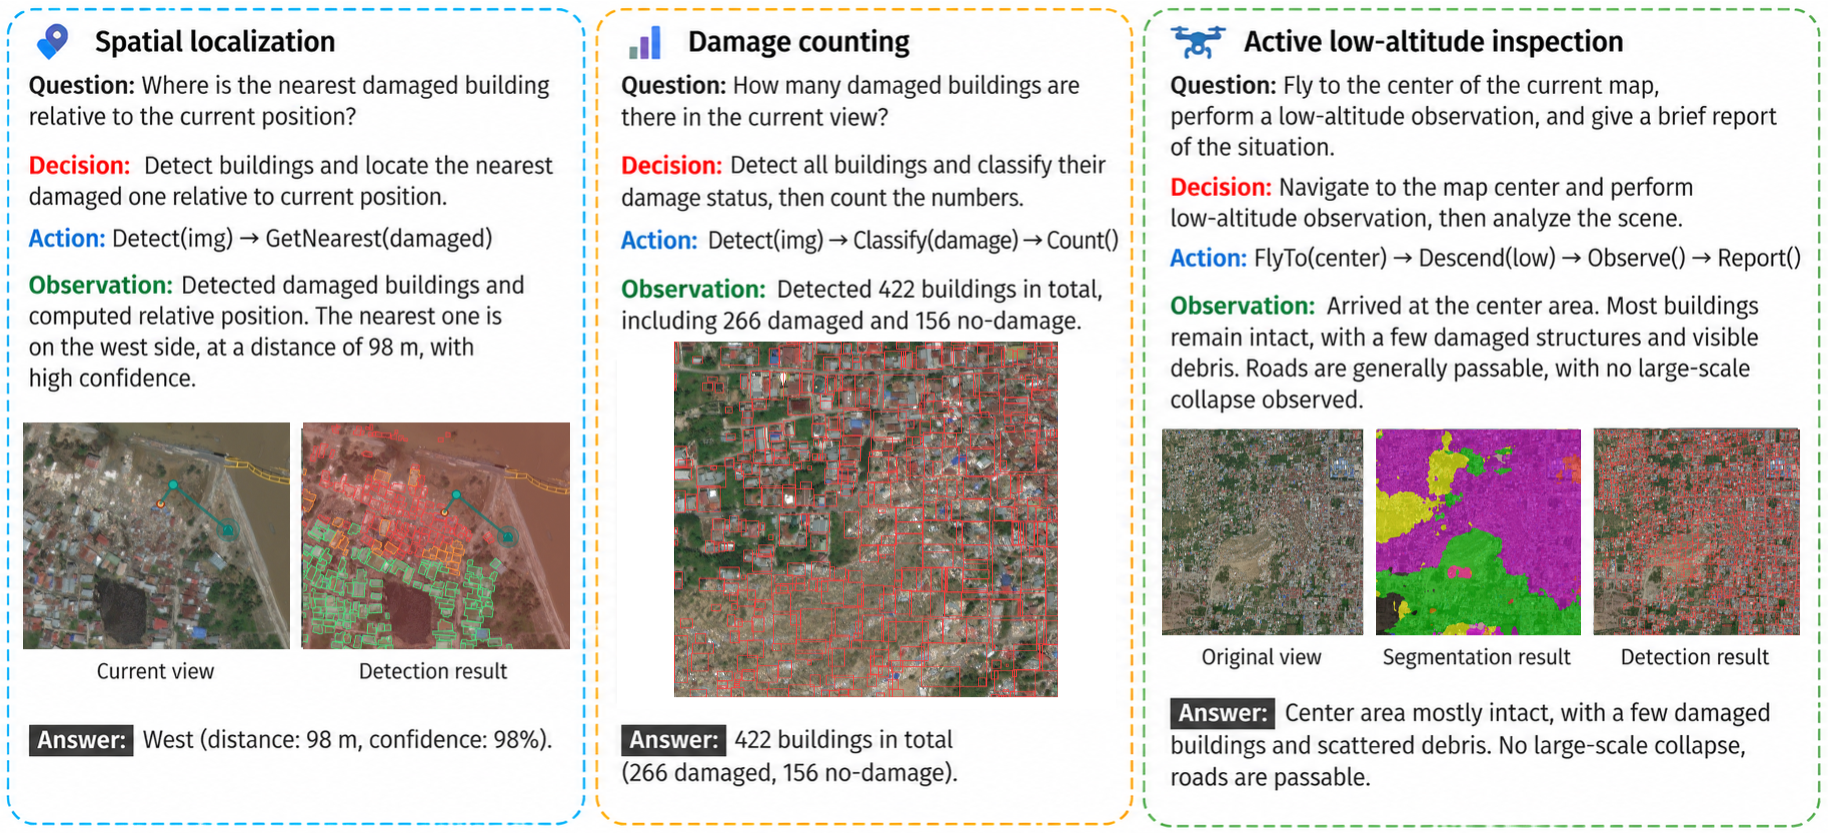
\includegraphics[width=\textwidth]{figure-paper/真正的输入输出.png}
\caption{Representative platform-run input--output traces. The examples show spatial localization from mapped detections, aggregation for damage counting, and an active low-altitude inspection sequence. They illustrate the interface and action vocabulary; quantitative results use the separately frozen benchmark and headless runner.}
\label{fig:task-traces}
\end{figure*}

\subsection{Final-set composition and input boundary}
The frozen set has 160 questions over 44 ROIs: 48 in Hurricane Michael, 51 in the Moore tornado, and 61 in Nepal flooding. Table~\ref{tab:answer-distribution} reports the answer counts. The count task is concentrated in $0$ and $3+$, with only one $1$ and no $2$; this class imbalance prevents count accuracy alone from establishing performance across all four categories. Spatial answers are more dispersed, but that task also requires finding the correct nearest damaged building. Questions from the same ROI share image context and therefore do not represent independent scenes.

\begin{table}[htbp]
\centering\small
\caption{Frozen question and answer distribution. Counts refer to distinct questions, before policy runs or generation repeats.}
\label{tab:answer-distribution}
\begin{tabularx}{\linewidth}{@{}l r X@{}}
\toprule
Task & $n$ & Reference answers (count)\\
\midrule
Presence & 44 & yes 30; no 14\\
Damage & 44 & damaged 29; no damage 15\\
Count & 43 & $0$: 14; $1$: 1; $2$: 0; $3+$: 28\\
Spatial & 29 & N 3; NE 4; E 3; SE 4; S 3; SW 3; W 4; NW 5\\
\bottomrule
\end{tabularx}
\end{table}

The source task record separates runtime inputs from scoring information. The controller receives the question, answer choices, ROI bounds, initial state, and a marked reference ID and coordinate only for a damage question. It receives detector-predicted boxes, probabilities, and geographic projections after observation. The reference answer, xBD damage labels and polygons, and the true nearest-damaged-building coordinate for a spatial question are restricted to benchmark construction and scoring. For spatial questions, the agent must select a target from predicted evidence because the ground-truth target coordinate is withheld.

Eligible records require usable post-disaster imagery, a geographic footprint, and building labels; pre-disaster imagery supplies the archival damage reference. The generator excludes consumed development tiles, checks answer vocabulary, geometry, duplicate records, and split membership, and retains ambiguity flags for review. The final questions underwent human review before the set was frozen. These checks document reference construction and the input boundary. Visual answerability and potential shortcuts require separate evaluation. Section~\ref{sec:results} therefore evaluates text-only and permitted-metadata controls on the same frozen set. The comparison assesses whether the complete image-aware pipeline outperforms controls using the permitted non-image inputs. Because the controls also use a modality-specific prompt and omit the hybrid rule path, the contrast does not isolate the causal effect of image access alone.

\section{Task-conditioned observation policy}
\label{sec:agent}
\subsection{Episode state and evidence memory}
An episode begins with a question $q$, geographic ROI, initial state $s_0=(x_0,y_0,h_0)$, and fixed reference answer $y_q$. At step $t$, the renderer produces $I_t=\mathcal{R}(\mathcal{M},s_t)$; ChangeOS supplies predicted building locations and binary damage probabilities, and the hybrid answer pipeline using Qwen2.5-VL-7B-Instruct proposes an answer. The controller can answer, abstain, search, or request a dedicated recheck. The normalized terminal answer is scored against $y_q$, with abstentions counted as incorrect for the primary endpoint. Every policy uses the same frozen ChangeOS checkpoint and answer path.

Predicted objects are projected into geographic coordinates. For non-damage tasks, sightings are associated when their predicted centers are within 6 m or their geographic boxes have intersection-over-union at least 0.2; damage sightings use the public marked-building reference ID. Each track retains observation IDs and averages binary probabilities with inverse-GSD weights. Count and spatial answers use tracks detected in the current observation, so a stale historical detection cannot independently supply a current nearest target. The memory may still merge nearby buildings or miss objects, even when geometric ROI coverage is high.

\subsection{Task-conditioned recheck rule}
For a candidate recheck, T1\_TASK uses
\begin{equation}
 U_q=u_q(1-h_{t+1}/h_t)-0.05\,\widehat{T}_{\mathrm{move}}/60
 -(1-\widehat{C}_{\mathrm{ROI}}),
 \label{eq:taskutility}
\end{equation}
where $u_q\in[0,1]$ is a task-specific uncertainty score, $\widehat{T}_{\mathrm{move}}$ is configured-speed motion time in seconds, and $\widehat{C}_{\mathrm{ROI}}$ is predicted coverage after the move. A candidate executes only when $u_q\geq0.5$, $U_q\geq0.05$, and, for count or spatial questions, predicted ROI coverage is at least 0.98. Only descent contributes positively to the utility. The rule therefore triggers descent subject to task uncertainty and coverage constraints; it neither assigns value to same-height viewpoint changes nor estimates calibrated accuracy gains.

The uncertainty score is defined separately for each task. For damage, it is normalized binary entropy for the marked predicted building; a visible marked location with no matched detection receives $u_q=1$. For count, a capped Poisson-binomial distribution from detected buildings' damage probabilities gives entropy over $0,1,2,3+$. For a matched spatial candidate, the score is the maximum of its binary entropy and a GSD-dependent estimate of proximity to an eight-sector bearing boundary. Presence is answered from the wide view when possible; missing evidence enters search rather than a local recheck. Count uncertainty is conditional on detected objects and does not account for missed buildings. The spatial score uses a selected predicted target and does not fully represent uncertainty about which damaged building is nearest.

Damage rechecks may move toward the marked building by at most 40 m horizontally and descend. Count and spatial rechecks keep the geographic center and descend only while the task ROI remains covered. Each active policy has a cap of two dedicated rechecks. The stored policy identifier A0\_HOLD is referred to here as \emph{A0\_NO\_RECHECK}: it has a zero dedicated-recheck cap but, like the other policies, may use up to six search steps. Search may move and render a new image. Thus A0\_NO\_RECHECK is not a fixed-view control, and the reported recheck count is not total movement, rendering, or model-call cost.

The primary comparators are A1\_RANDOM (a seeded 0.5 recheck trigger), A2\_ALWAYS (request a feasible recheck), and A3U\_RAW\_ENTROPY (uncalibrated binary-entropy trigger). A3\_ENTROPY and A4\_CONFORMAL are supplemental policies. All seven configurations share the same question set and search cap, but their executed actions and subsequent answer-call counts may differ. This comparison therefore measures whole-policy outcomes at their realized operating points.

\section{Evaluation protocol}
\label{sec:setup}
The evaluation links changes in observation to building predictions and task answers. The development camera-ladder diagnostic compares cruise, intermediate, and floor observations for the same 7,238 annotated buildings in 43 ROIs. Its fixed-denominator measure counts unmatched ground-truth buildings as incorrect. Classification accuracy among matched buildings describes a selected subset and is not used as the task endpoint. This diagnostic helps interpret whether the rendered view changes available predicted evidence.

The final online set is separate from the 160-question development set used to select policy rules. Seven frozen policies each answer the same 160 final questions under three generation repeats, yielding $7\times160\times3=3{,}360$ episodes. The repeats vary seeded generation conditions for the same questions; they do not increase the number of independent questions, ROIs, or events. The primary endpoint is terminal question accuracy, with abstentions counted incorrect. Executed dedicated rechecks, within-policy answer transitions, task type, and event are descriptive companion measures.

We audited spatial separation beyond distinct tile IDs. The 43 development ROIs and 44 final ROIs share no tile ID or xBD building UID (0 shared among 7,238 and 4,963 eligible ROI buildings), but 9/1,892 cross-set ROI pairs intersect; the maximum ROI IoU is 0.461 and the maximum fraction of the smaller ROI covered by the other is 0.631. Comparing 129 centered development camera-ladder footprints with all 802 recorded T1 final observation footprints across three repeats, 1,871/103,458 cross-set pairs intersect. The maximum footprint IoU is 0.882, and one smaller footprint lies entirely inside a larger one (overlap fraction 1.000). These measurements identify overlapping geographic windows but do not establish whether both sets contain the same xBD pixels or physical buildings. Different tiles may assign different UIDs to the same physical structure. Thus question and tile disjointness does not establish spatial independence.

We add two controls on the frozen final set. First, the task-majority baseline predicts one answer per task type using a question/ROI-disjoint development set. S1\_LANGUAGE receives question text, choices, and task type; S2\_METADATA additionally receives runtime-visible ROI bounds/tile, initial pose, and, for damage questions, the permitted marked-building reference and coordinate. Both exclude images, detector outputs, annotation labels and polygons, the reference answer, and the spatial true-nearest target. S1 and S2 use the same Qwen checkpoint, answer vocabulary, generation settings, seed schedule, and exact-match scoring as the main answer model, but a modality-appropriate text-only JSON prompt and no hybrid rule path.

Second, a fixed-view matched-call diagnostic is run at every one of the 161 executed T1 dedicated rechecks. Immediately before the live recheck, the fixed branch clones the semantic map and evidence memory, remains at the old pose, reruns perception on the old view, and calls the ordinary hybrid answer path. The changed branch executes the logged action, perceives the new view, and calls that same answer path. The two branches share question, repeat, next-step seed, model, and generation settings; their prompts differ only through the resulting predicted evidence. A strict gate requires a byte-identical fixed-branch marked image and exactly one fixed and changed model call with the shared seed. The diagnostic compares paired candidate answers immediately after the transition, without following both branches to episode termination. The fixed-branch answer is never used by the T1 controller.

Four T1\_TASK contrasts were specified before the final run: against A0\_NO\_RECHECK (internal identifier A0\_HOLD), A1\_RANDOM, A2\_ALWAYS, and A3U\_RAW\_ENTROPY. Comparisons pair the same question and repeat. The 5,000-draw bootstrap resamples ROI clusters, retaining their questions and repeats, and reports Bonferroni-adjusted 98.75\% intervals for the four contrasts. The intervals characterize uncertainty across the 44 observed ROI clusters. The three-event sample does not support inference about transfer to unseen disasters. Task and event breakdowns are descriptive, not additional adjusted tests.

For the matched diagnostic, correctness pairs and answer disagreement are summarized overall and by task, with a 5,000-draw ROI-cluster bootstrap 95\% interval for the changed-minus-fixed difference. Shortcut results report overall and task-wise accuracy; image-aware A0\_NO\_RECHECK and T1 gaps to S1/S2 are paired by question and repeat with the same ROI-cluster bootstrap. These controls assess visual dependence and observation value and are not used for additional policy selection.

The primary cost count records executed dedicated rechecks. Search can also move and render, and policies can make different numbers of later Qwen calls; total movement, rendering, perception, and generation costs are therefore not summarized by the recheck column. A supplementary archive audit reports observation and generation-attempt counts, search actions, state-derived movement on complete trajectories, and episode wall time (Table~\ref{tab:cost-audit}). Episode wall time is measured software runtime, not flight duration. The final protocol identifies the frozen task, model, prompt, and run configurations; the audit scope and planned release are summarized in \ref{app:provenance}. A runnable single-episode scene and scoring replay is described in \ref{app:minimal-reproduction}.

\section{Results and discussion}
\label{sec:results}

\subsection{Image-aware performance and shortcut controls}
The final answer distribution yields a strong task-majority baseline: the development-fitted task-majority rule attains 57.50\% (92/160). This result reflects the frozen answer distribution, particularly for count questions, without using visual evidence. The text-only S1\_LANGUAGE control reaches 28.75\% over 480 question--repeat instances, and the permitted-metadata S2\_METADATA control reaches 36.25\% (Table~\ref{tab:shortcut-controls}). Neither control receives imagery or detector evidence. In contrast, the image-aware A0\_NO\_RECHECK and T1\_TASK operating points reach 72.29\% and 75.00\%, respectively. Their paired gaps to S1 are $+43.54$ and $+46.25$ points, and to S2 are $+36.04$ and $+38.75$ points; all four 95\% ROI-cluster intervals exclude zero. The complete image-aware pipelines therefore outperform the evaluated controls based on question wording and permitted non-image metadata. Because S1/S2 also use a modality-specific prompt and omit the hybrid rule path, the comparison measures a pipeline-level difference and does not isolate the causal effect of image access.

\begin{table*}[!t]
\centering\small
\caption{Shortcut controls and image-aware operating points on the frozen final set. S0 uses a development-fitted task majority and is deterministic ($n=160$); all other rows use three aligned repeats ($n=480$). S1 receives question text, choices, and task type; S2 additionally receives permitted runtime metadata.}
\label{tab:shortcut-controls}
\resizebox{\textwidth}{!}{%
\begin{tabular}{lcccrrrrr}
\toprule
Method & Image & Detector evidence & Runtime metadata & Presence & Damage & Count & Spatial & Overall\\
\midrule
S0 task majority & no & no & task only & 68.18 & 65.91 & 65.12 & 17.24 & 57.50\\
S1 language only & no & no & question only & 31.82 & 34.09 & 32.56 & 10.34 & 28.75\\
S2 metadata only & no & no & permitted & 31.82 & 58.33 & 32.56 & 14.94 & 36.25\\
\midrule
A0\_NO\_RECHECK & yes & yes & permitted & 93.18 & 66.67 & 75.97 & 43.68 & 72.29\\
T1\_TASK & yes & yes & permitted & 93.18 & 75.76 & 78.29 & 41.38 & 75.00\\
\bottomrule
\end{tabular}}
\end{table*}

\subsection{Observation changes under matched answer calls}
The policy comparison alone cannot distinguish a new image from another answer opportunity. We therefore created paired branches at all 161 executed T1 rechecks, with each pair sharing its pre-recheck state. The fixed branch reran perception and answering on the previous view. The changed branch executed the original recheck before perception and answering. The strict validity gate accepted all 161 pairs, with no missing pair or execution error. The branch schedule reproduced the original recheck-step locations in 118 of 119 episodes; the one mismatch retained the same two rechecks but placed the second at a different step, reflecting re-runnable perception-path variation.

The changed-view branch produces correct candidate answers in 96/161 transitions (59.63\%), versus 81/161 (50.31\%) for the fixed-view matched call, a paired difference of $+9.32$ points (95\% ROI-cluster interval $[-2.00,+21.74]$). The point estimate is accompanied by 36 fixed-wrong/changed-correct transitions and 21 fixed-correct/changed-wrong transitions; 44 pairs are wrong in both branches and 60 correct in both. Answers disagree in 42.24\% of pairs. Thus the changed observation can alter the answer path beyond a repeated call on the old image, but the clustered interval does not establish a stable positive average effect in the sampled ROIs.

Excluding the one episode whose rerun placed its second recheck at step 2 rather than reference step 3 removes two wrong--wrong pairs. The remaining 159 pairs from 118 episodes have 81/159 fixed-view and 96/159 changed-view correct candidates, a $+9.43$-point paired difference (95\% ROI-cluster interval $[-2.03,+22.00]$), with the same 36 help and 21 harm transitions. As a separate old-view repeat check, the pre-recheck and fixed-branch image bytes and normalized candidate answers agree in all 161/161 original forks (159/159 after exclusion). The two old-view calls use different step seeds and evidence prompts, however, so this is observed answer stability under identical image bytes rather than a controlled same-prompt, same-seed repeatability estimate.

\begin{table}[htbp]
\centering\small
\caption{Fixed-view matched-call diagnostic at executed T1 recheck transitions. Candidate-answer correctness is measured immediately after the branch, not at episode termination. Presence has no T1 dedicated recheck.}
\label{tab:matched-view}
\begin{tabular}{lrrrrrr}
\toprule
Task & $n$ & Fixed & Changed & Help & Harm & $\Delta$ pp\\
\midrule
Damage & 123 & 46.34 & 58.54 & 27 & 12 & $+12.20$\\
Count & 18 & 83.33 & 100.00 & 3 & 0 & $+16.67$\\
Spatial & 20 & 45.00 & 30.00 & 6 & 9 & $-15.00$\\
\midrule
Overall & 161 & 50.31 & 59.63 & 36 & 21 & $+9.32$\\
\bottomrule
\end{tabular}
\end{table}

Figure~\ref{fig:help-harm-cases} grounds the aggregate transitions in two frozen T1 episodes. In the damage episode \nolinkurl{hurricane-michael_00000435_post_disaster__damage_0001_9430}, successive observations at approximately 1330, 887, and 443~m increase the marked building's predicted damage probability from 0.158 to 0.369 and 0.588. The answer consequently changes from the incorrect ``no damage'' to the correct ``damaged.'' This example illustrates the potential benefit of a more local observation for a damage question.

In contrast, the spatial episode \nolinkurl{hurricane-michael_00000306_post_disaster__spatial_0092_5452} shows the complementary risk. The wide observation selects a damaged building north of the ROI center and answers correctly. After descent, the evidence ranking selects a different building southwest of the center, changing a correct answer to an incorrect one. A further descent is rejected because predicted ROI coverage is 0.340, below the 0.98 gate. The failure involves a change in target identity under reduced regional context, rather than only bearing noise for a fixed target.

\begin{figure*}[!t]
\centering
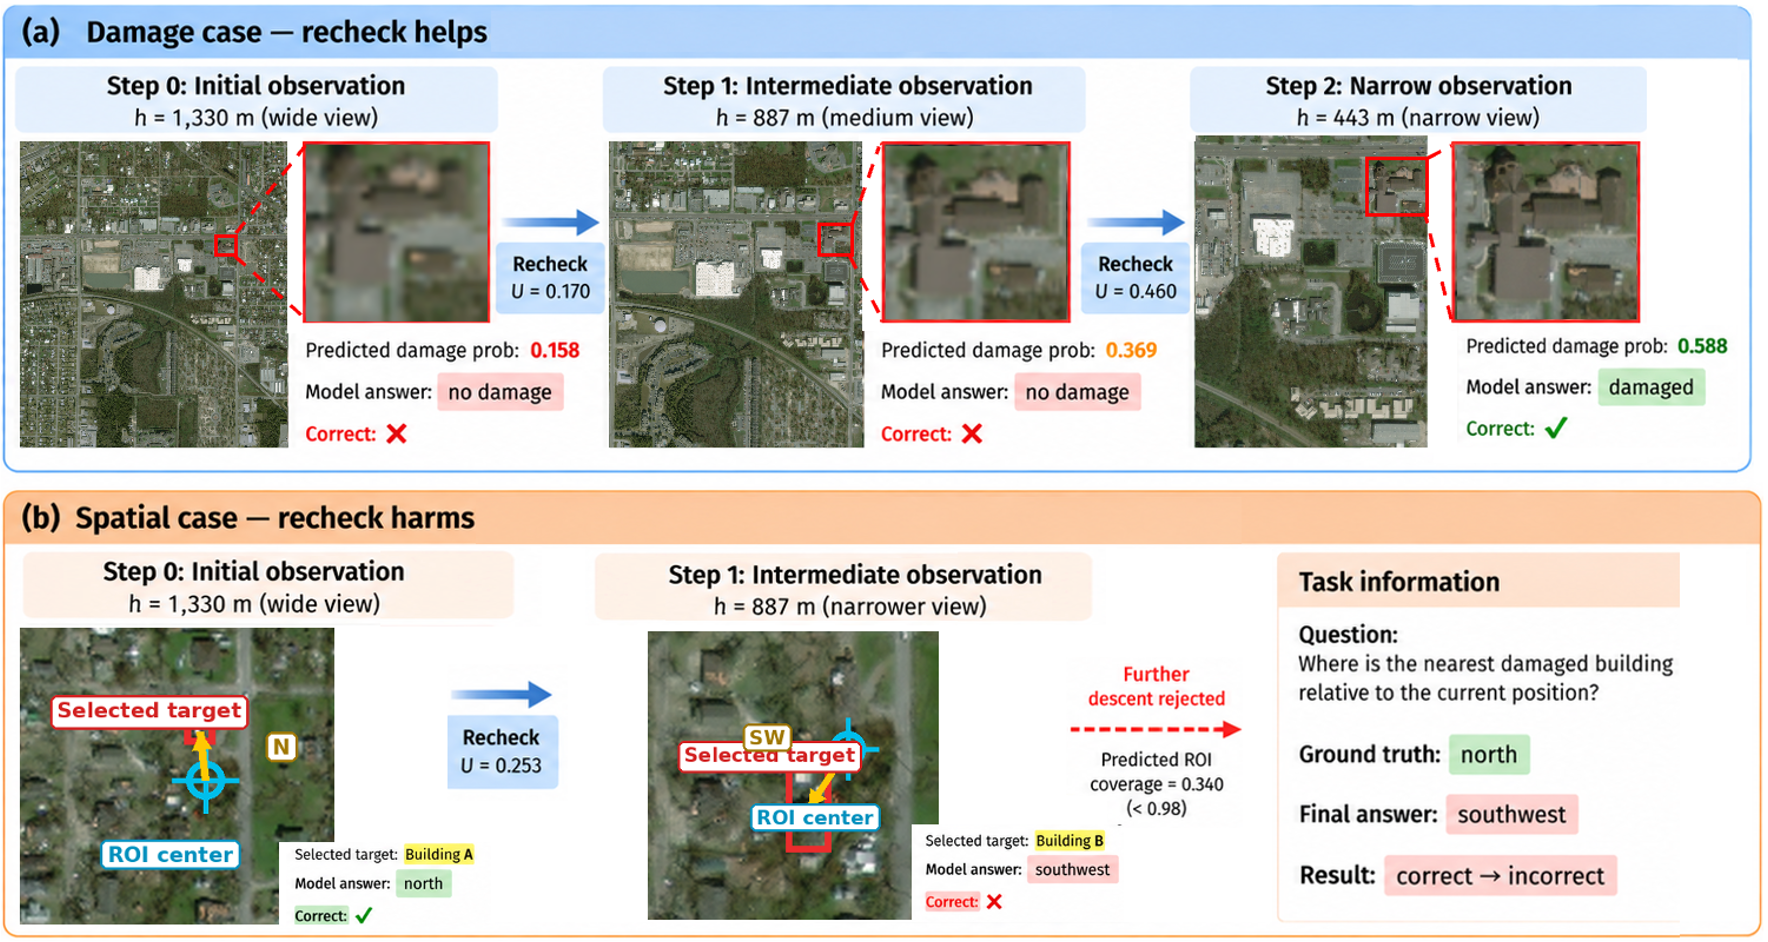
\includegraphics[width=\textwidth]{figure-paper/recheck成功失败两个案例.png}
\caption{Frozen examples of recheck help and harm. (a) Narrower observations strengthen evidence for a marked building and correct a damage answer. (b) A spatial recheck changes the selected nearest damaged building from the correct northern target to a southwestern target; the coverage gate then rejects further descent. The examples expose the action--observation--evidence--answer chain behind the aggregate help and harm counts.}
\label{fig:help-harm-cases}
\end{figure*}

\subsection{Building-level evidence and task-dependent outcomes}
The camera-ladder diagnostic holds 7,238 annotated buildings in 43 development ROIs fixed while changing the rendered footprint. ChangeOS localization recall rises from 22.09\% at cruise to 34.06\% at intermediate and 56.52\% at floor. With every unmatched ground-truth building counted as incorrect, binary building accuracy rises from 20.01\% to 31.06\% and 53.65\%. Among matched buildings only, binary damage accuracy is 90.56\%, 91.20\%, and 94.92\%, while matched-only macro-F1 is 0.8714, 0.8743, and 0.9232. The paired cruise-to-floor outcomes include 2,696 incorrect-to-correct changes and 261 correct-to-incorrect changes. The building-level diagnostic shows that rendering changes affect the predicted evidence available to the agent. Asymmetric pre-/post-image processing and changes in context prevent attributing these effects solely to GSD or physical descent.

Table~\ref{tab:detection-fp-audit} separates localization from conditional damage classification. Localization precision falls to 68.65\% at floor even as recall and matched-building damage accuracy rise; unmatched predictions increase to 43.44 per ROI. TP/FP/FN use a one-to-one nearest-centroid match within 12~m, so an unmatched prediction can reflect a duplicate, localization error, or missing annotation as well as a spurious building. The all-GT accuracy denominator includes missed buildings but does not penalize extra predictions; matched-only accuracy and macro-F1 exclude misses and unmatched predictions. The gains in damage accuracy and the increase in localization false positives thus describe different aspects of the detection pipeline.

\begin{table*}[!t]
\centering\small
\caption{ChangeOS localization and binary-damage audit on the same 43 development ROIs and 7,238 annotated buildings at each height. Loc. P/R are localization precision/recall; FP is an unmatched prediction, FN an unmatched GT building, and FP/ROI is FP/43. All-GT accuracy counts unmatched GT as wrong but does not count unmatched predictions; matched accuracy and macro-F1 condition on matched GT only.}
\label{tab:detection-fp-audit}
\resizebox{\textwidth}{!}{%
\begin{tabular}{lrrrrrrrrr}
\toprule
View (height) & TP & FP & FN & Loc. P (\%) & Loc. R (\%) & FP/ROI & All-GT acc. (\%) & Matched acc. (\%) & Matched macro-F1\\
\midrule
Cruise (1330 m) & 1,599 & 502 & 5,639 & 76.11 & 22.09 & 11.67 & 20.01 & 90.56 & 0.8714\\
Intermediate (887 m) & 2,465 & 677 & 4,773 & 78.45 & 34.06 & 15.74 & 31.06 & 91.20 & 0.8743\\
Floor (443 m) & 4,091 & 1,868 & 3,147 & 68.65 & 56.52 & 43.44 & 53.65 & 94.92 & 0.9232\\
\bottomrule
\end{tabular}}
\end{table*}

The matched-call results show that task answers also respond differently to observation changes. Damage and count transitions have positive point differences, whereas spatial transitions have a negative point difference (Table~\ref{tab:matched-view}). A more local view can improve the evidence for a marked building or a damaged-count decision, yet it can change the selected target for a nearest-building direction judgment. These task-wise estimates are descriptive because T1 selects the recheck subsets, which contain only 18 count and 20 spatial transitions.

\subsection{Complete-policy performance}
Table~\ref{tab:final-policies} reports the prespecified complete-policy runs. T1\_TASK has the highest observed terminal accuracy, 360/480 question--repeat instances (75.00\%), with 161 executed dedicated rechecks. A0\_NO\_RECHECK (the internal configuration identifier is A0\_HOLD) forbids dedicated rechecks but permits search and answers 347/480 (72.29\%). A2\_ALWAYS makes 923 rechecks and answers 307/480 (63.96\%). Active policies share a maximum of two dedicated rechecks. Their realized operating points differ in actions, model calls, and total cost, which are not matched in this comparison.

\begin{table}[htbp]
\centering\small
\caption{Primary frozen policy operating points on the same 160 questions under three generation repeats. Rechecks are executed dedicated actions and exclude search.}
\label{tab:final-policies}
\begin{tabular}{lrrr}
\toprule
Policy & Correct / 480 & Accuracy (\%) & Rechecks\\
\midrule
A0\_NO\_RECHECK & 347 & 72.29 & 0\\
A1\_RANDOM & 326 & 67.92 & 419\\
A2\_ALWAYS & 307 & 63.96 & 923\\
A3U\_RAW\_ENTROPY & 339 & 70.63 & 626\\
T1\_TASK & 360 & 75.00 & 161\\
\bottomrule
\end{tabular}
\end{table}

The 2.71-point T1\_TASK advantage over A0\_NO\_RECHECK is an observed difference of 13 correct question--repeat instances, not 13 distinct questions. Its 98.75\% multiplicity-adjusted interval includes zero (Table~\ref{tab:final-contrasts}), as does the comparison with raw entropy. The positive interval against A2\_ALWAYS supports a difference between these complete policies on the sampled ROIs; it does not show that T1's individual changed observations caused that difference.

\begin{table}[htbp]
\centering\small
\caption{Prespecified paired T1\_TASK terminal-accuracy contrasts in percentage points. The 98.75\% ROI-cluster intervals adjust for four comparisons.}
\label{tab:final-contrasts}
\begin{tabular}{lrr}
\toprule
Contrast & Difference & 98.75\% interval\\
\midrule
T1 minus A0\_NO\_RECHECK & $+2.71$ & $[-2.04,+7.50]$\\
T1 minus A1\_RANDOM & $+7.08$ & $[+0.01,+14.69]$\\
T1 minus A2\_ALWAYS & $+11.04$ & $[+0.86,+21.38]$\\
T1 minus A3U\_RAW\_ENTROPY & $+4.38$ & $[-4.33,+12.96]$\\
\bottomrule
\end{tabular}
\end{table}

At the terminal-episode level, presence is unchanged between T1 and A0\_NO\_RECHECK, damage and count are numerically higher for T1, and spatial accuracy is lower (Table~\ref{tab:shortcut-controls}). Performance also varies by event: T1 versus A0 is 54.86\% versus 58.33\% in Hurricane Michael, 84.31\% versus 77.12\% in Moore, and 83.06\% versus 79.23\% in Nepal. Together, the matched-call results and complete-policy comparisons characterize task-dependent corrections and harms. The interval for the A0 contrast and incomplete cost measurements limit conclusions about the overall effectiveness and efficiency of the recheck policy.

\section{Limitations}
\label{sec:limitations}
The benchmark contains 44 ROIs from three events, and questions from nearby regions may share image context. Although development and final questions use distinct tiles and building UIDs, their ROIs and rendered footprints can overlap geographically. Together with the fixed ChangeOS checkpoint's prior xBD exposure, these overlaps limit claims of spatial independence and transfer to unseen disasters. The final answer distribution is uneven, particularly for count questions. The image-aware pipelines substantially outperform the evaluated shortcut controls, but this result does not establish that every question requires visual evidence or exclude unmeasured shortcuts. Human review and deterministic annotation rules support reference construction without guaranteeing visual answerability for every question.

The camera ladder resamples orthographic imagery and uses asymmetric pre-/post-disaster processing. It cannot reproduce changes in viewing angle, occlusion, acquisition conditions, or motion dynamics during physical descent. The spatial uncertainty score is conditional on a selected predicted target and does not fully capture uncertainty about which damaged building is nearest. The target switch in Fig.~\ref{fig:help-harm-cases} illustrates this unresolved source of harm.

A0\_NO\_RECHECK permits search, and policies may differ in subsequent answer-call counts. The matched-call diagnostic controls for an additional answer opportunity at recheck transitions but does not follow both branches to episode termination. Perception may remain nondeterministic under identical image pixels, and the 95\% ROI-cluster interval for the matched-call difference includes zero. The old-view agreement check varies prompts and seeds, so it does not exclude model variance under strictly identical calls. The qualitative examples illustrate observed mechanisms without establishing a generally positive recheck effect.

Recheck counts exclude search and do not capture total rendering, perception, generation, or flight costs. Of the 3,360 episodes, 42 lack a recorded state after the terminal fly action. This omission affects complete-motion summaries but leaves the terminal-answer denominator unchanged.

\section{Conclusion}
DisasterClaw contributes an evaluation component for embodied UAV intelligence: it keeps the geographic scope and reference answer fixed while the agent's action changes the observation. Its episode records connect actions, predicted building evidence, answer calls, and terminal outcomes. The four task families capture a trade-off between local detail and regional coverage that building-classification accuracy alone does not describe.

On the frozen final set, image-aware pipelines outperform the evaluated text-only and permitted-metadata controls. At matched recheck transitions, changed observations yield more corrections than harms, but the ROI-cluster interval for the average difference includes zero. The task-wise point estimates are positive for damage and count and negative for spatial questions. T1\_TASK achieves the highest observed complete-policy accuracy, although its adjusted contrast with the search-enabled A0\_NO\_RECHECK policy also includes zero. In the full MESSI release, existing single-temporal YOLO and SegFormer models were connected to DisasterClaw's evidence and recheck controllers for 409 vegetation regions. The action-enabled arm used 20 lower views and answered 372/409 correctly, compared with 369/409 for paired hold; six answers were corrected and three harmed. On the same 20 triggered cases, an equal-budget repeat-high arm answered 12/20 correctly and the real-low arm answered 15/20, isolating the second-view contribution from the additional answer opportunity. A supplementary random-selection control with the same 20-recheck budget averages 369.20/409 over 20 fixed seeds (range 367--371), below the entropy trigger's 372/409. This supports selective allocation on the evaluated cohort; the seed spread does not establish cross-scene generalization. The 34 IrYamim Test regions had appeared in earlier Qwen-only explorations and are not an untouched holdout; both current arms answer 25/34 correctly. These results show that an adapted controller can gate access to new observations in a real-image offline replay. The net gain is small, and physical flight, vehicle dynamics, and transfer of the unchanged disaster-damage pipeline remain untested.

\section*{Declarations}
\noindent\textbf{Acknowledgements and funding.} \textit{To be supplied by the authors, including funder names, grant numbers, and relevant contributions. No absence of funding is asserted.}

\smallskip\noindent\textbf{CRediT author statement.} \textit{To be assigned and approved by the named authors.}

\smallskip\noindent\textbf{Declaration of competing interest.} \textit{To be confirmed by all authors.}

\smallskip\noindent\textbf{Data and code availability.} We will release the DisasterClaw code, benchmark task definitions, frozen protocols, audited episode traces, analysis scripts, and a runnable minimal reproduction package with its example xBD tile and labels on GitHub. The repository will provide environment instructions, file checksums, and instructions for obtaining the full xBD imagery and model checkpoints from their respective sources. The planned release repository is \url{https://github.com/emmmmmmnbbb/DisasterClaw}. This availability statement describes the intended release; completeness of the public archive remains to be verified before submission.

\smallskip\noindent\textbf{Generative AI assistance.} Generative AI tools were used to assist manuscript restructuring, English-language editing, reference checking, and preparation of analysis and typesetting scripts. The authors are responsible for the scientific claims, experimental design, reported results, and final manuscript content. \textit{Author confirmation of this disclosure and final review is required before submission.}

\appendix
\setcounter{table}{0}
\renewcommand{\theHtable}{A.\arabic{table}}
\section{Protocol and provenance}
\label{app:provenance}
The frozen execution protocol identifies the final task set and consolidated human-review report, three-event manifest, ChangeOS checkpoint, source fingerprint, prompt, policy configuration, and analysis scripts by SHA-256. The planned GitHub release will include the protocol, task and scene manifests, dependency specifications, replay instructions, and verified links to the original imagery and checkpoint sources.

The final run consists of 12 shards with 3,360 question--policy--repeat rows. The shard audit reports complete question and configuration coverage and zero execution errors. This checks execution consistency, not independent reconstruction of the full environment. A separate cost audit finds that 42 episodes end with a fly action and no subsequent recorded state; complete-motion summaries therefore use 3,318 episodes. The terminal-answer analysis retains all 3,360. Search-action detail and component-level render, perception, controller, and Qwen costs are not available, so the action-cost comparison is restricted to executed dedicated rechecks and observed episode wall time.

The supplementary-control report aggregates 12 matched-view shards (161 valid forks, no missing pairs or execution errors) and four shortcut shards (960 valid text-only or metadata-only predictions, no call errors or invalid outputs). The planned GitHub release will include the machine-readable report, task-wise counts, ROI-cluster intervals, and protocol notes describing the fixed-view branch, allowed shortcut fields, and diagnostic boundaries. It will also include the matched-view and shortcut-control runners and the report-generation script so these results can be regenerated from the released inputs.

For the camera-ladder diagnostic, the construction boundary is summarized below. The table is a reproducibility description, not an ablation of preprocessing choices.
\begin{table}[htbp]
\centering\small
\caption{Camera-ladder preprocessing construction used by the diagnostic.}
\label{tab:preprocessing-construction}
\begin{tabularx}{\linewidth}{@{}lXX@{}}
\toprule
Stage & Pre-disaster & Post-disaster\\
\midrule
Geographic crop & matched window & current footprint\\
Scale handling & assumed source scale & footprint-dependent sampling\\
Alignment & paired affine placement & paired affine placement\\
Detector input & retained source-scale channel & resized current view\\
\bottomrule
\end{tabularx}
\end{table}

\section{Minimal frozen episode reproduction}
\label{app:minimal-reproduction}
\setcounter{table}{0}
\renewcommand{\theHtable}{B.\arabic{table}}
The planned GitHub release will include a minimal example that replays one frozen T1\_TASK damage episode, \nolinkurl{hurricane-michael_00000435_post_disaster__damage_0001_9430}, generation repeat 0. The example contains the paired $1024\times1024$ xBD tile images, the post-disaster polygon/UID annotations, a scene manifest with geographic ROI and pixel-to-geographic transform, a compact record of the episode's observations and actions, a standard-library Python replay script, and exact expected output. SHA-256 digests in the manifest detect asset substitution. This example can be run without detector or language-model weights; it reproduces scene linkage, observation-window geometry, the archived action trace, and reference-answer scoring, but does not rerun perception or generation.

The environment for this replay is Python 3.11 with no third-party packages. The GitHub README will specify how to run the replay script and compare its output with the expected result. For fresh model inference, the release will provide full environment specifications, the frozen task and review manifests, and instructions for obtaining the ChangeOS and Qwen2.5-VL-7B-Instruct checkpoints. A fresh inference run need not reproduce the archived candidate sequence exactly.

The replay first verifies the two image hashes and their dimensions, locates the marked building by xBD UID in the post-disaster label, and computes its binary damage reference from the original \texttt{major-damage} subtype. It then constructs each observation footprint from the recorded pose using the $60^\circ$ field of view and the same geographic conversion used by the renderer. Table~\ref{tab:minimal-episode-trace} gives the compact recorded action sequence. The final \texttt{Report} answer is compared with the annotation-derived reference, yielding the expected output \texttt{reference=damaged}, \texttt{answer=damaged}, and \texttt{correct=true} (the underlying task vocabulary is Chinese). The example identifies its source frozen record by question ID, generation repeat, and shard.

\begin{table}[htbp]
\centering\small
\caption{Expected trace of the single frozen damage episode. Candidate answers are shown in English for readability; the replay emits the original Chinese labels.}
\label{tab:minimal-episode-trace}
\begin{tabular}{@{}rlll@{}}
\toprule
Step & Height (m) & Candidate & Action\\
\midrule
0 & 1330.22 & no damage & Fly/reobserve\\
1 & 886.82 & no damage & Fly/reobserve\\
2 & 443.42 & damaged & Report\\
\bottomrule
\end{tabular}
\end{table}

The GitHub release will also include a supplementary audit script and its machine-readable output. The script reads the matched-call shards, development camera-ladder report, both frozen question manifests, xBD labels, and final T1 traces. Its output contains the schedule-exclusion calculation, old-view answer agreement, building-UID and geographic overlap audit, and the TP/FP/FN counts in Table~\ref{tab:detection-fp-audit}. No new model inference is needed for these audit calculations.


\subsection{MESSI archived scoring and fresh inference}
The existing MESSI archive has separate entry points for rescoring recorded outcomes and rerunning perception. From the repository root, \texttt{python3} followed by \nolinkurl{experiments/messi_case/scripts/score_single_temporal_agent.py} recomputes the three-stratum hold/agent summary. The corresponding \nolinkurl{experiments/messi_case/scripts/score_trigger_repeat_control.py} checks the triggered IDs and shared initial predictions and recomputes the equal-budget repeat-high versus real-low comparison. These scripts read the archived episodes and separate reference manifests; they do not rerun the models or validate fresh-inference reproducibility.

Fresh inference uses \nolinkurl{experiments/messi_case/scripts/run_single_temporal_agent.py} with \texttt{--split} set separately to \texttt{full\_descend}, \texttt{full\_train\_paths}, and \texttt{full\_test\_paths}, and \texttt{--device} selecting the available device. The matched repeat-high runs additionally use \texttt{--triggered-repeat-high}. Input preparation, model requirements, and run ordering are documented in \nolinkurl{experiments/messi_case/single_temporal_agent_protocol.md}. This route requires the prepared MESSI crops and model weights; the archived scoring route requires the episode logs and reference manifests. Local entry points do not establish completeness of the planned public release.


The random-budget supplement is specified in \nolinkurl{experiments/messi_case/supplement_random_budget/protocol.md}; its frozen selection manifest defines all 20 seeds. GPU traces, model provenance, and per-seed results are stored under \nolinkurl{experiments/messi_case/supplement_random_budget_gpu/}. The entry \nolinkurl{experiments/messi_case/scripts/score_random_budget_supplement.py} recomputes the comparison from these records without inference. Fresh runs use \nolinkurl{experiments/messi_case/scripts/run_random_budget_gpu.sh} with a device argument such as \texttt{cuda:0}. The separate \nolinkurl{scripts/benchmarks/report_supplement_costs.py} audits the frozen benchmark calls, geometric motion, and software wall times reported in Table~\ref{tab:cost-audit}.

\begingroup\small
\bibliographystyle{elsarticle-num}
\bibliography{references,messi_case}
\endgroup
\end{document}
